\documentclass[11pt]{article}
\textwidth166mm
\textheight232mm
\oddsidemargin00mm
\topmargin-20mm

\usepackage{graphicx}
\usepackage{epsfig}
\usepackage{hyperref}
\usepackage{textcomp}
\usepackage{subcaption}
%\usepackage{natbib}
\usepackage{enumitem}
%\setlength{\bibsep}{1pt plus 0.3ex}
%\usepackage{biblatex}

\newcommand{\chandra}{{\it Chandra}}
\newcommand{\rxte}{{\it RXTE}}
\newcommand{\asca}{{\it ASCA}}
\newcommand{\rosat}{{\it ROSAT}}
\newcommand{\einstein}{{\it EINSTEIN}}
\newcommand{\ginga}{{\it GINGA}}
\newcommand{\bbxrt}{{\it BBXRT}}
\newcommand{\suzaku}{{\it Suzaku}}
\newcommand{\xmm}{{\it XMM-Newton}}
\newcommand{\sax}{{\it BeppoSAX}}
\newcommand{\ec}{$\eta$~Car}
\newcommand{\glast}{{\it Fermi}}
\newcommand{\swift}{{\it Swift}}
\newcommand{\integral}{\textit{INTEGRAL}}
\newcommand{\nustar}{\textit{NuSTAR}}
\newcommand{\hst}{{\it HST}}
\newcommand{\ms}{$M_{\odot}$}
\newcommand{\rs}{$R_{\odot}$}
\newcommand{\ls}{$L_{\odot}$}
\newcommand{\kms}{km~s$^{-1}$}
\newcommand{\fluxcgs}{erg\,cm$^{-2}$\,s$^{-1}$}
\newcommand{\lumcgs}{erg~s$^{-1}$}
\newcommand{\hgps}{H.E.S.S. galactic plane survey}
\newcommand{\hess}{HESS~J1844-030}
\newcommand{\lat}{{\it Fermi}-LAT}
\newcommand{\cxo}{CXO~J1845-031}
\newcommand{\fl}{FLY8~J1844.7-0304}
\newcommand{\twomass}{2MASS~J18444178-0305522}
%CXO~J184441.7-030549
%CXO J184441.7-030549
%Fermi data: $2.94\pm0.83 \times 10^{-11}$\,\fluxcgs. 
%Curvature: $4.23\sigma$. 
%Significance: $7.169\sigma$.



\begin{document}
	
	\begin{center}
		\rule[0.2cm]{16.6cm}{0.1cm}
		\large{\bf Observing Proposal 2017/2018}
		\rule[0.2cm]{16.6cm}{0.1cm}
	\end{center}
		
	{\bf 1. Background}

	The goal of this memo is to estimate the expected number of photons from a heavy ion received at the end of a wavelength shifting fiber (WLS) by a Hamamatsu S1330-3050VS (or the newer model) SiPM based on previous empirical results.
	
	The estimation is done in two parts: the creation of simulated light curves using previous empirical data to generate putative probability density functions for various physical processes, and an estimation of the energy deposition by heavy ions in CsI (Sodium dopping ignored).
	
	{\bf 2. Scintillation Simulation}
	
	Previously, a collimated 662 keV gamma-ray beam from a Cs-137 source was directed downward through the top of the APT imagining calorimeter prototype. A typical (if not slightly bright) example trace is shown in Figure \ref{fig:CsI_trace}. Collection of scintillation pulses at the WLS fiber ends where done with a Tektronix TDK 3052 oscilloscope. Due to this fact, only one channel was observed at a time but provided excellent capture resolution and low electronic noise (although burst-like noise was present in the system).
	
	Due to Fig. \ref{fig:CsI_trace}'s clean profile it was chosen to be the basis the WLS photon arrival-time PDF. The PDF was created by taking the oscilliscope trace and smoothing its profile via a low-tolerance b-spline representation (Fig. \ref{fig:CsI_PDF}). The resulting profile was then interpolated so that the total array length was 10,000.
	
	A similar process was done for the the amplitude of the WLS fiber photon's voltage signals. The system was allowed to run, but triggered on (e.g. traces collected) the individual SiPM photonelectron signals. An overplot of 1,200 of such signals is shown in Figure \ref*{fig:PE_traces} and Figure \ref{fig:PE_traces_hist} shows their voltage distribution. The histogram in Figure \ref{fig:PE_traces_hist} was the basis of the photoelectron PDF (Figure \ref{fig:PE_traces_PDF}). Some of the larger signals were clipped, but do not represent a large fraction of the total events. The data were captured while studying different preamplifier designer and the oscilliscope settings were a compromise between the different design's
	signal amplitude.
	
	The time profile of the photoelectron pulses was modeled as a Gaussian with a FWHM $\approx$ 20 ns. An example of the simulated trace with 50 photons is shown in Figure \ref{fig:example_trace}. The quiescent noise is modeled as Gaussian white noise.

	{\bf 2. Energy Deposition Estimation}
	
	Energy deposition was estimated using Bethe equation:
	\begin{center}
		\begin{equation}
			-\frac{dE}{dx}=4\pi N_{A} r_{e}^{2} \frac{m_{e}c^{2}}{\beta^{2}}[\frac{1}{2}\ln(\frac{2 \gamma^{2}\beta^{2}m_{e}c^{2}E_{max}}{I_{0}^{2}})-\beta^{2}-\frac{\epsilon}{2}-\frac{\delta(\beta\gamma)}{2}]
		\end{equation}
	\end{center}

	Shell and energy corrections were not included in the calculation. The shell correction is applicable at low energies ($<$ 1 MeV). The density correction was not included because I can not find its functional form anywhere I look, despite constant reference to it.
	
	Figure \ref{fig:stopping} shows the calculated stopping power for liquid water and CsI. The calculated values are in good agreement with NIST values (Table \ref{table:stopTable}).
	
	Using Equation 1, the energy deposition from a ion moving through 5 mm of CsI is approximated. This is done by choosing an initial incident energy, $E_0$, and calculating its energy loss by moving through a small length of the scintillator, $\Delta x$,An incident ion with
	
	\begin{table}
		
		\centering
		\begin{tabular}{c c c}
			\hline\hline
			Energy [$MeV$]  & NIST Stopping Power [$MeV cm^{2} g^{-1}$] & Mine [$MeV cm^{2} g^{-1}$] \\
			\hline
			10 & 4.021 & 4.064 \\
			100 & 1.317 & 1.331 \\
			1000 & 1.412 & 1.473 \\
			\hline
		\end{tabular}
		\caption{Calculated and reference stopping power for CsI at various energies.}
		\label{table:stopTable}
	\end{table}
	
	
	
	
	\begin{figure}
		\centering
		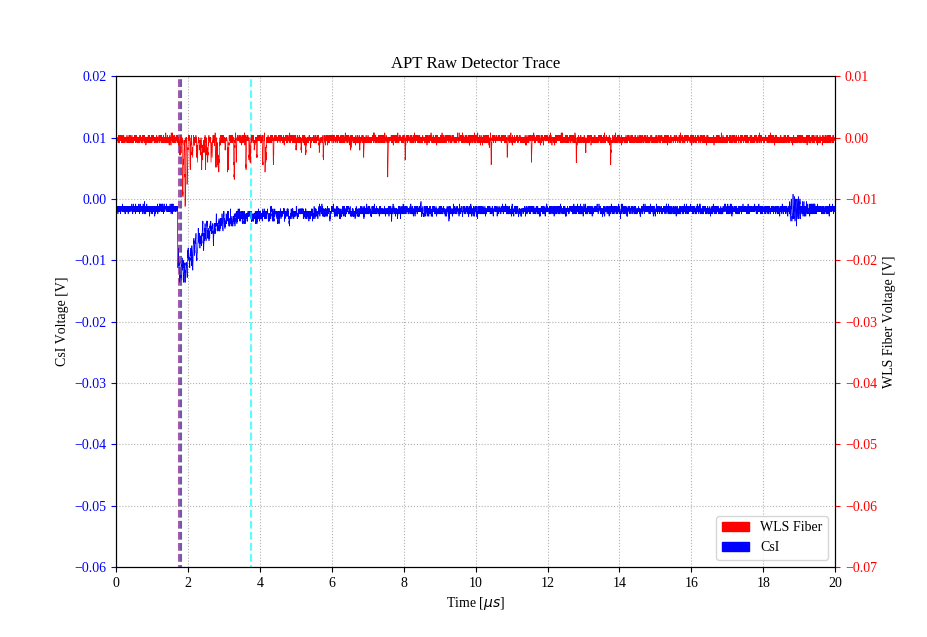
\includegraphics[width=1.0\linewidth]{CsI_trace}
		\caption{A well-defined 662 keV trace from Cs-137 (ostensibly). It was chosen for its clean profile, though some noise is present near 19 $\mu s$.}
		\label{fig:CsI_trace}
	\end{figure}

	\begin{figure}
		\centering
		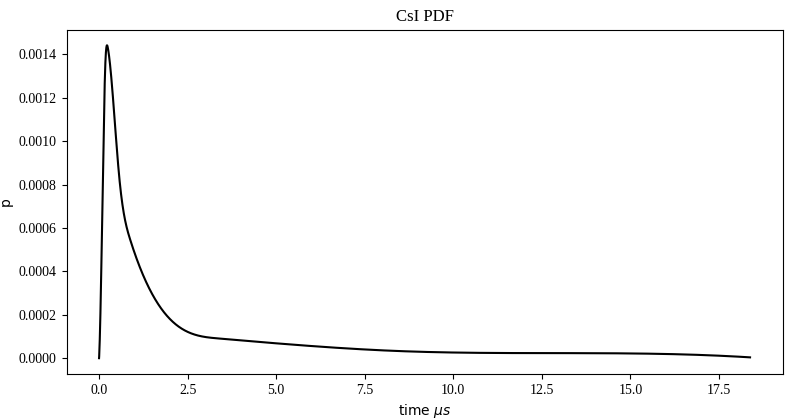
\includegraphics[width=1.0\linewidth]{CsI_PDF}
		\caption{The smoothed, normalized trace of Fig. \ref{fig:CsI_trace}.}
		\label{fig:CsI_PDF}
	\end{figure}

	\begin{figure}
		\centering
		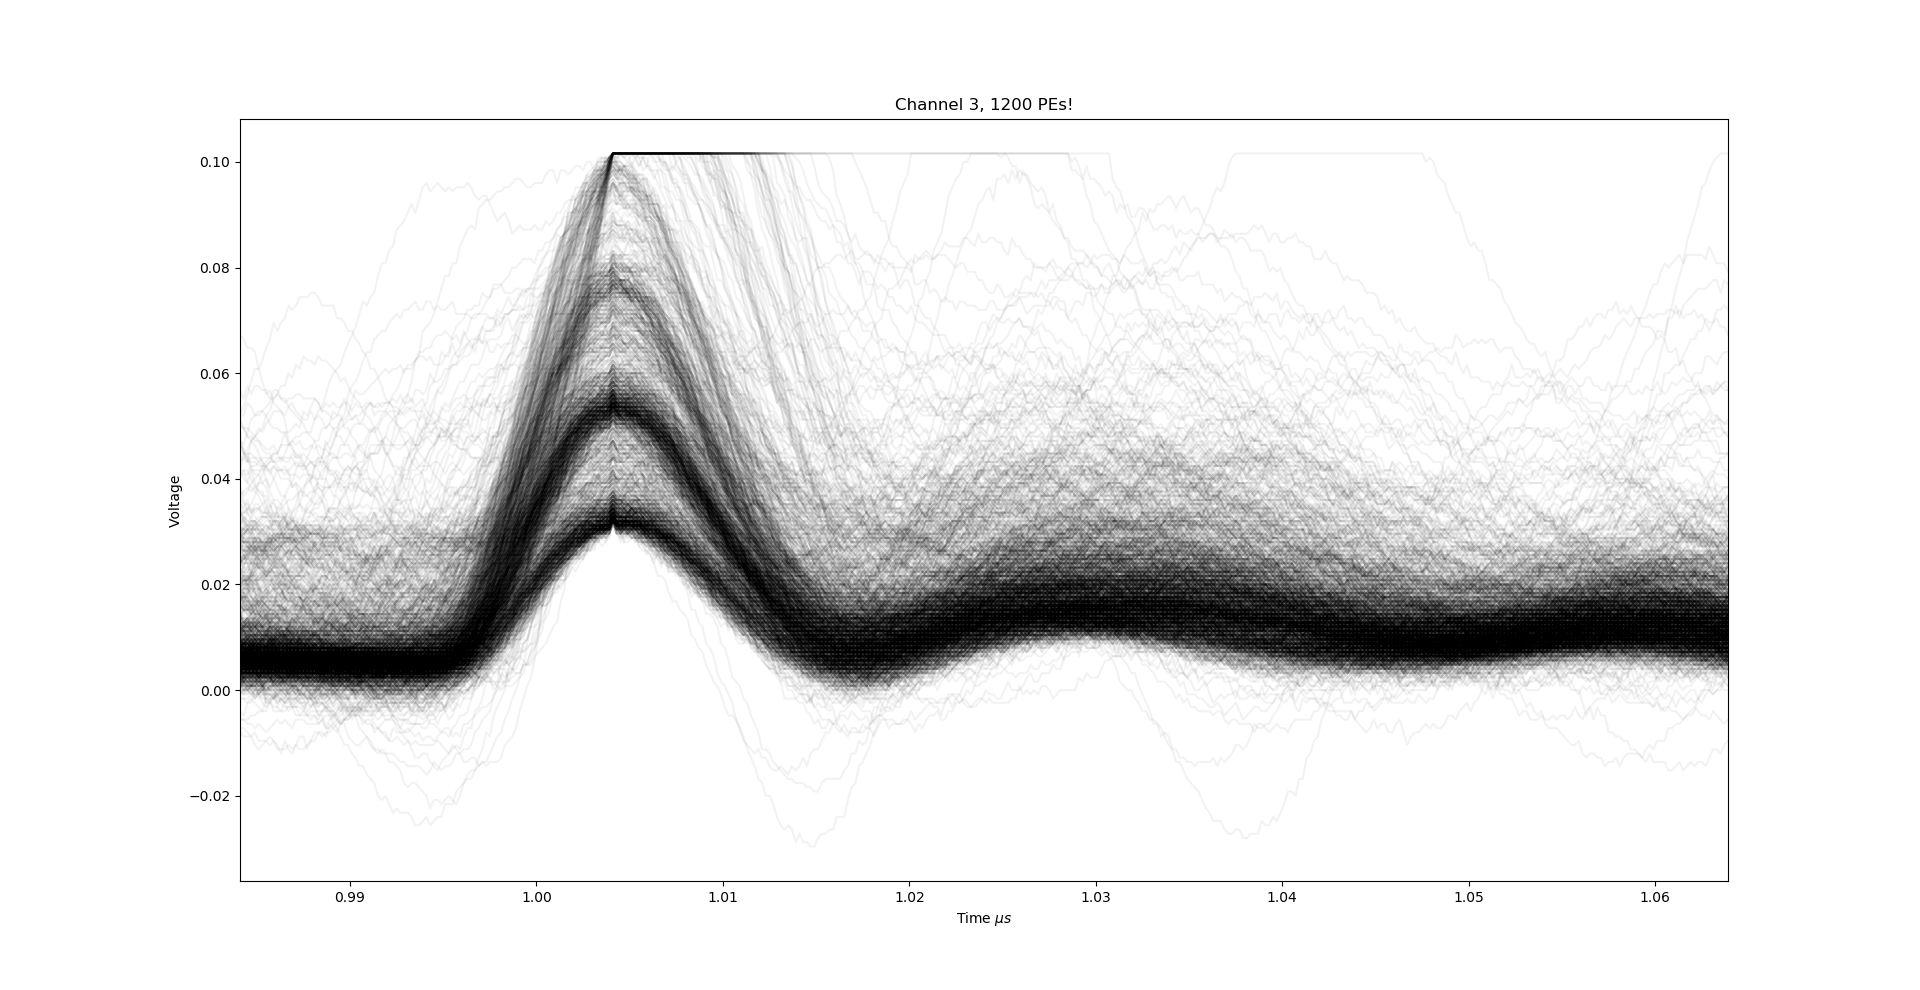
\includegraphics[width=1.2\linewidth]{1200_channel3_PEs}
		\caption{Overplot of 1,200 photoelectron events from the third SiPM channel.}
		\label{fig:PE_traces}
	\end{figure}

	\begin{figure}
		\centering
		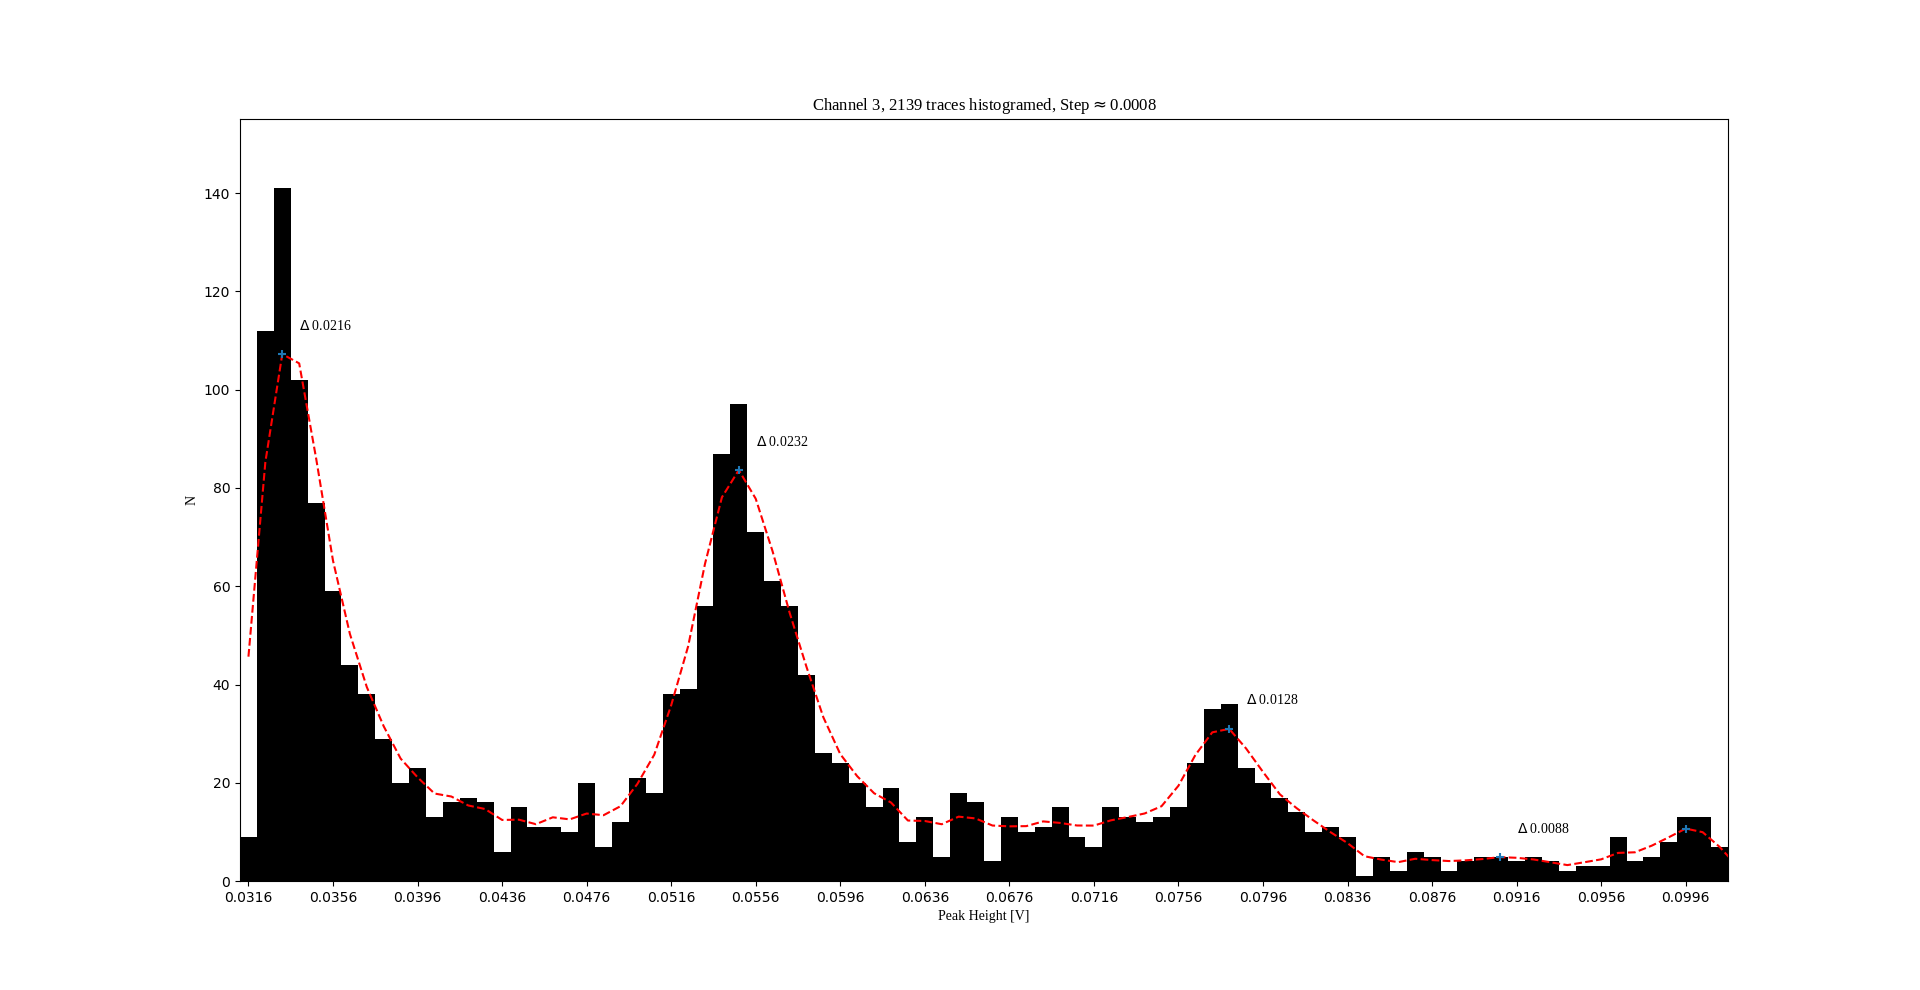
\includegraphics[width=1.0\linewidth]{1200_channel3_PEs_hist_diff}
		\caption{Voltage distribution of signals shown in Figure \ref{fig:PE_traces}.}
		\label{fig:PE_traces_hist}
	\end{figure}

	\begin{figure}
		\centering
		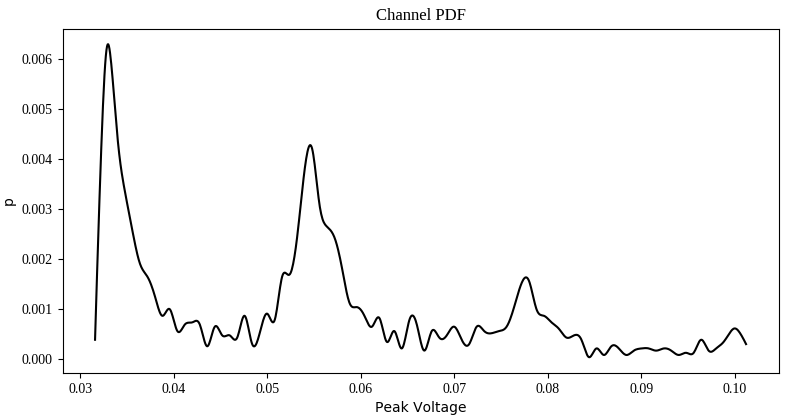
\includegraphics[width=1.0\linewidth]{1200_channel3_PEs_PDF}
		\caption{The smoothed, normalized profile of Figure \ref{fig:PE_traces_hist}.}
		\label{fig:PE_traces_PDF}
	\end{figure}

	\begin{figure}
		\centering
		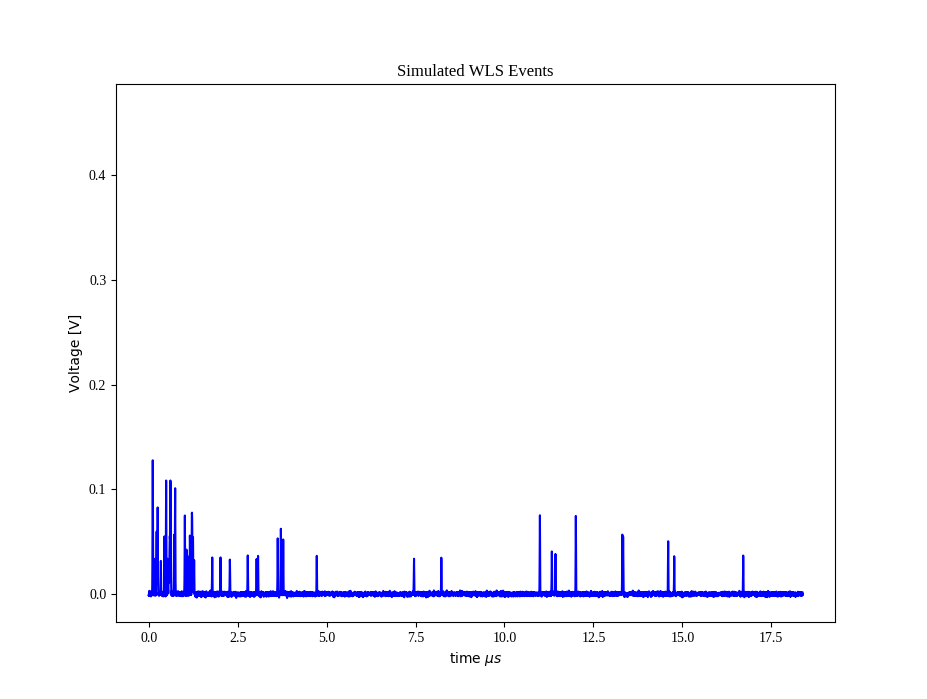
\includegraphics[width=1.0\linewidth]{example_trace}
		\caption{Simulated WLS fiber SiPM response to 50 photons.}
		\label{fig:example_trace}
	\end{figure}

	\begin{figure}
		\centering
		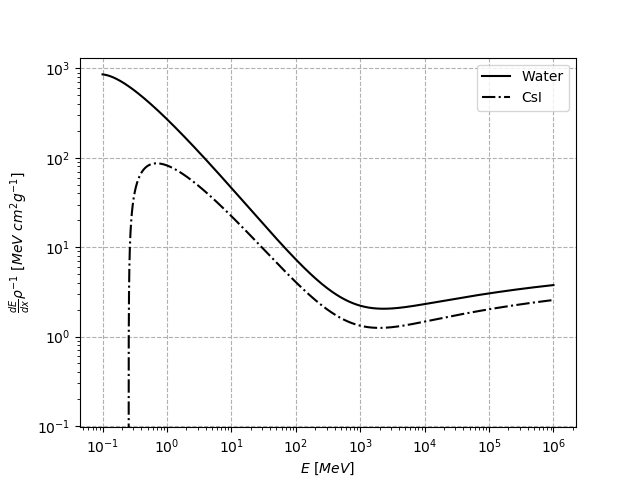
\includegraphics[width=1.0\linewidth]{stopping}
		\caption{Calculated stopping power of liquid water and CsI}
		\label{fig:stopping}
	\end{figure}

	
	%
	\begin{thebibliography}{99}
		\bibitem{Aharonian2005b}Aharonian, F. A., et al. 2005, A\&A, 442, 1
		
		\bibitem{Dubus2015b} Dubus, G. 2015, CRPhy, 16, 661
		
		\bibitem{Dubus2013} Dubus, G. 2013, A\&ARv, 21, 64
		
		\bibitem{Chang} Z. Chang, S. Zhang, et al. 2016, $Mon.Not.Roy.Astron.Soc.$ 463 no.1, 495-501
		
		\bibitem{hessposter} Christoph Deil. 2015. url: \url{https://indico.cern.ch/event/344485/contributions/1744018/attachments/1136486/1626371/HESS_HGPS_ICRC2015_Deil.pdf}.
		
		\bibitem{hess} H. E. S. S. Collaboration et al. A\&A 612, A1 (2018).
		
		\bibitem{grin} V. Grinberg et al. A\&A 608, A143 (2017).
		
		\bibitem{Helfand} D. J. Helfand et al. ApJ341 (1989).
		
		\bibitem{radio} G. Castelletti et al. A\&A 602, A31 (2017).
		
	\end{thebibliography}
\end{document}

